\documentclass[aspectratio=169,11pt]{beamer}
\usetheme{Madrid}
\usecolortheme{seahorse}
\usepackage{booktabs}
\usepackage{graphicx}
\usepackage{amsmath}
\usepackage{hyperref}
\graphicspath{{../visualize/figures/}{../pipeline/outputs/figures/}}
\setbeamertemplate{navigation symbols}{}
\setbeamertemplate{footline}{}

\title[Dengue Surge Warning]{Can Recent Surveillance and Weather Data\\Flag Dengue Surge Risk?}
\subtitle{Singapore, weekly forecasts}
\author{Tran Duy Tai\\Do Nhat Thanh\\Nguyen Thi Quynh Thu}
\institute{42.510\\Statistical Learning}
\date{December 2026}

\begin{document}

\begin{frame}
  \titlepage
\end{frame}

\begin{frame}{Decision question}
  \begin{block}{For Singapore dengue surveillance teams}
    Can information available by week $t$ help identify a materially elevated
    dengue fever (DF) week at $t+h$?
  \end{block}
  \begin{itemize}
    \item Forecast horizons: 1, 2 and 4 weeks
    \item Compare recent cases, weather, and their combination
    \item Predictive association only; this is not a causal estimate or live alert
  \end{itemize}
\end{frame}

\begin{frame}{Why is an early warning difficult?}
  \begin{itemize}
    \item Dengue is endemic, but incidence and outbreak timing vary substantially.
    \item Recent counts are powerful, but can make a model look good through persistence.
    \item Weather may add useful lead time, but the weather sources disagree.
    \item A false alarm consumes response capacity; a missed surge delays preparation.
  \end{itemize}
  \vspace{0.4em}
  \begin{alertblock}{Key distinction}
    Predicting that an ongoing high period continues is not the same as warning before onset.
  \end{alertblock}
\end{frame}

\begin{frame}{Data: national cases plus local weather}
  \begin{columns}[T]
    \column{0.53\textwidth}
      \begin{itemize}
        \item MOH weekly bulletin, 2012--2022 (574 epi weeks)
        \item Target: Dengue Fever; DHF kept separate (rare)
        \item NEA/MSS Changi (S24): rainfall and temperature
        \item Open-Meteo: humidity; checked against NEA monthly RH
        \item MOH epi weeks mapped to the following Monday
      \end{itemize}
    \column{0.43\textwidth}
      \begin{itemize}
        \item 0 duplicated or missing case weeks
        \item MOH releases identical for 209/261 DF weeks
        \item Max revision: 8 cases/week; totals differ by 0.2\%
        \item Weather agreement: temperature $r=0.91$, rain $r=0.48$
      \end{itemize}
  \end{columns}
\end{frame}

\begin{frame}{Three meanings of a surge}
  Let $y_t$ be weekly DF cases and $h$ the horizon:
  \begin{enumerate}
    \item \textbf{Threshold A:} $y_{t+h}>\text{mean}_{52,t}+2\text{SD}_{52,t}$
    \item \textbf{Seasonal S:} above the historical same-season 90th percentile
    \item \textbf{Growth G:} at least 50 cases and a 25/30/45\% rise for $h=1/2/4$
  \end{enumerate}
  \vspace{0.4em}
  Onset A/S only count weeks when the current series is not already above threshold.
  At $h=1$, A--S Jaccard overlap is 0.31; S--G is 0.05.
\end{frame}

\begin{frame}{What goes into the models?}
  \begin{itemize}
    \item Case history: log counts, lags, rolling means, recent growth
    \item Season: week-of-year and Fourier terms
    \item Weather: rain, rain days, temperature and humidity at lags 0--12 weeks
  \end{itemize}
  \begin{block}{Model families}
    Prior, seasonal and persistence baselines; logistic regression (cases/weather/full);
    lasso logistic; CART; random forest; Poisson GLM; ridge on log counts.
  \end{block}
  Count forecasts are converted to probabilities of crossing each surge threshold.
\end{frame}

\begin{frame}{Validation: respect time and label availability}
  \begin{itemize}
    \item Expanding-window rolling origin by week; evaluation begins in 2016.
    \item Refit weekly; purge examples whose full label horizon is not yet known.
    \item Development outcomes are before 2022; final-period outcomes are in 2022.
    \item Earlier observed 2022 labels can enter training for later rolling forecasts.
    \item Metrics: PR-AUC, precision, recall, Brier/calibration, alarms/year;
    count MAE/RMSE in cases/week.
    \item 95\% moving-block bootstrap intervals (26-week blocks).
  \end{itemize}
  \begin{alertblock}{Important qualification}
    Earlier exploratory runs included forecasts through 2022. This is not a pristine
    static test set; describe it as a final-period prequential check.
  \end{alertblock}
\end{frame}

\begin{frame}{Development results ($h=1$, target weeks 2016--2021)}
  \centering\small
  \begin{tabular}{l r c l c c}
  \toprule
  Target & Pos. & Persistence & Best model: PR-AUC [95\% CI] & P & R\\
  \midrule
  A threshold & 43 & 0.93 & Poisson GLM 0.93 [0.78, 0.98] & 0.62 & 0.93\\
  S seasonal & 44 & 0.97 & Ridge log-count 0.98 [0.77, 1.00] & 0.75 & 1.00\\
  G growth & 36 & 0.17 & Ridge log-count 0.26 [0.15, 0.40] & 0.22 & 0.53\\
  A-onset & 7 & 0.30 & Poisson GLM 0.32 [0.04, 0.80] & 0.17 & 0.57\\
  S-onset & 5 & 0.26 & Ridge log-count 0.89 [0.70, 1.00] & 0.33 & 1.00\\
  \bottomrule
  \end{tabular}
  \vspace{0.5em}
  \begin{itemize}
    \item Level surges (A, S): persistence is as good as any model, so this is not early warning.
    \item Growth and S-onset: count regression beats the baselines, but S-onset has only 5 events.
    \item Weather-only logistic: 0.34 / 0.16 / 0.13, close to the base rates; adding weather does not help.
  \end{itemize}
\end{frame}

\begin{frame}{2022 final-period check}
  \begin{center}
    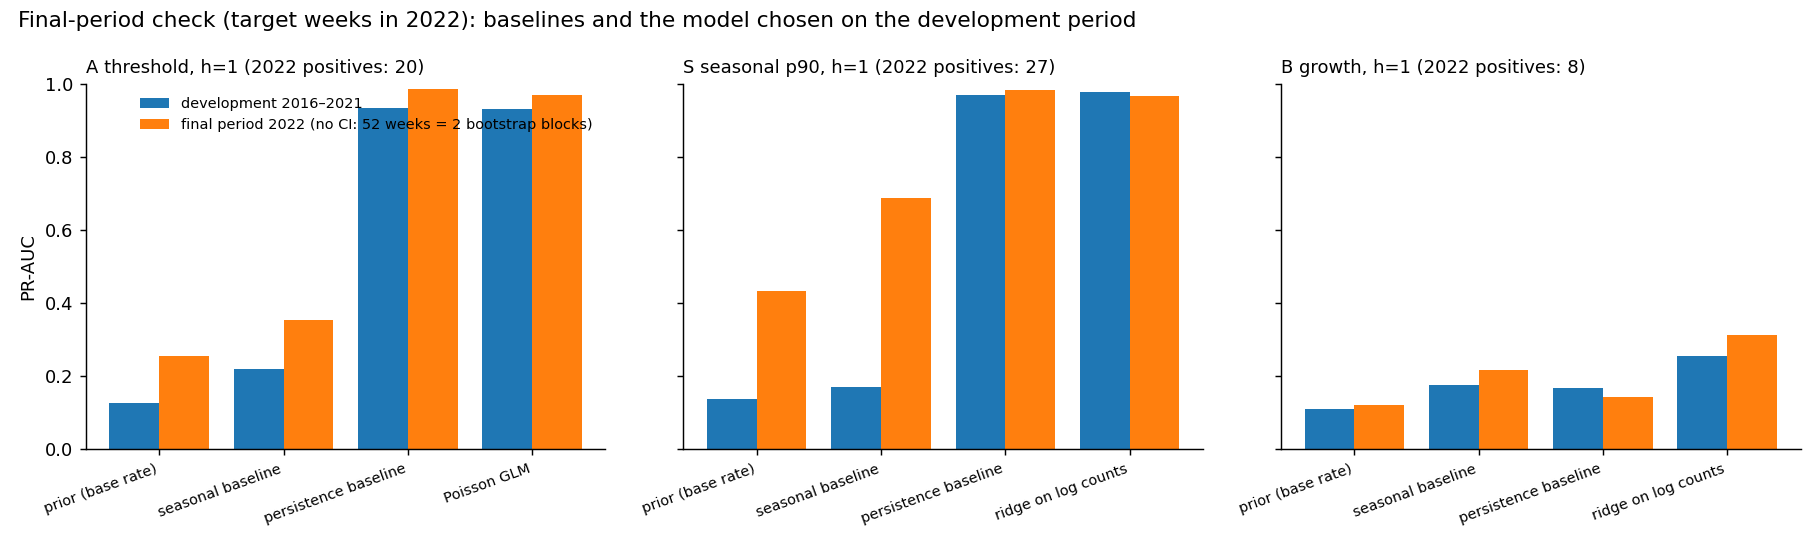
\includegraphics[width=0.95\linewidth]{12_final_test_holdout_h1.png}
  \end{center}
  \small
  Ranking holds: A/S persistence 0.98 vs selected model 0.97; growth 0.31 vs persistence 0.14
  (8 positives). Onset targets have only 2 positives in 2022, too few to compare models.
\end{frame}

\begin{frame}{Failure case: alarm at the 2022 peak}
  \begin{columns}[T]
    \column{0.58\textwidth}
      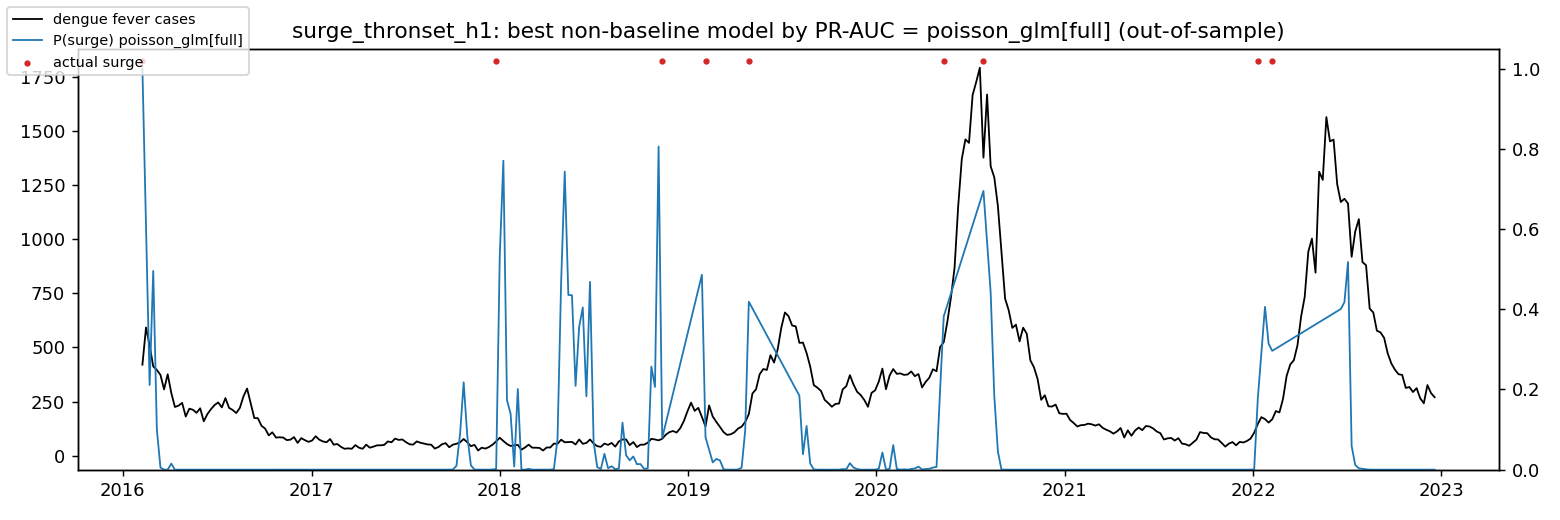
\includegraphics[width=\linewidth]{11_model_best_surge_thronset_h1.png}
    \column{0.40\textwidth}
      \small
      \begin{itemize}
        \item Target: A-onset, $h=1$; model: Poisson GLM
        \item Origin 2022-07-04: forecast 1{,}383 cases, $P=0.52$, so an alarm is raised
        \item Observed: 918 cases. The epidemic had peaked
        \item The model extrapolated recent growth into a turning point
        \item It also missed the 2022-01-17 onset ($P=0.18$, just below the 0.20 threshold)
      \end{itemize}
  \end{columns}
\end{frame}

\begin{frame}{Limitations and responsible use}
  \begin{itemize}
    \item Few outbreaks and very few onset positives mean wide uncertainty.
    \item No serotype, immunity, spatial exposure or local case counts.
    \item Notified cases can shift with testing and reporting; COVID-19 is a special period.
    \item One weather station and weaker rainfall/humidity agreement limit input quality.
    \item The assumed 4:1 cost ratio is illustrative, not elicited from decision-makers.
  \end{itemize}
  \begin{block}{Use}
    Retrospective research comparison only; never use these scores as deployed public-health
    alerts without prospective validation and human review.
  \end{block}
\end{frame}

\begin{frame}{Takeaways}
  \begin{enumerate}
    \item Surge definitions materially change the warning task.
    \item Persistence must be beaten before claiming useful early warning.
    \item Count regression helps for growth and onset surges, but few events mean wide intervals.
    \item Weather adds no measurable skill beyond recent counts at 1--4 weeks.
  \end{enumerate}
  \vspace{1em}
  \centering
  \Large Questions?
\end{frame}

\appendix
\begin{frame}{Reproducibility and team contributions}
  \begin{itemize}
    \item Pipeline, configuration, processed weekly snapshots and source manifest are included.
    \item Main run: \texttt{cd pipeline \&\& .venv/bin/python run.py all}
    \item AI-use disclosure: \texttt{AI\_USE.md}
    \item Contributions: \textcolor{red}{[to be completed by the group]}
  \end{itemize}
\end{frame}

\end{document}
